\documentclass[tikz]{standalone}
\usepackage{tikz}
\usepackage{../../../../glossary}
\usetikzlibrary{arrows.meta, chains, positioning}

\begin{document}

    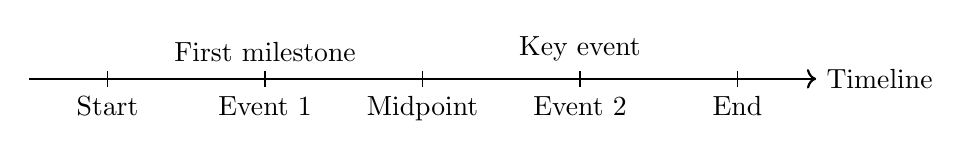
\begin{tikzpicture}[xscale=10] % Adjust xscale for A4 width

    % Draw the timeline
    \draw[->, thick] (0, 0) -- (1, 0) node[right] {Timeline};

    % Add ticks and labels (example)
    \foreach \x/\label in {0.1/Start, 0.3/Event 1, 0.5/Midpoint, 0.7/Event 2, 0.9/End} {
        \draw (\x, 0.1) -- (\x, -0.1); % Ticks
        \node[below] at (\x, -0.1) {\label}; % Labels
    }

    % Add example event descriptions above the timeline
    \foreach \x/\text in {0.3/First milestone, 0.7/Key event} {
        \node[above] at (\x, 0.1) {\text};
    }

    \end{tikzpicture}

\end{document}